\documentclass{article}
\usepackage[utf8]{inputenc}
\title{database systems the complete book chapter 2: the relational model of data}
\author{wbg231 }
\date{December 2022}
\newcommand{\R}{$\mathbb{R}$}
\newcommand{\B}{$\beta$}
\newcommand{\A}{$\alpha$}
\newcommand{\D}{\Delta}

\newcommand{\avector}[2]{(#1_2,\ldots,#1_{#2})}
\newcommand{\makedef}[2]{$\textbf{#1}$:#2 }
\usepackage{tikz,graphicx,hyperref,amsmath,amsfonts,amscd,amssymb,bm,cite,epsfig,epsf,url}

\begin{document}

\maketitle

\section{introduction}
\begin{itemize}
\item \href{https://people.inf.elte.hu/miiqaai/elektroModulatorDva.pdf}{reading link} that is the whole book, but we are only responsible for chapter 2 
\section{an overview of data models}
\item a data model is a notation for describing data consisting of three parts 
\begin{itemize}
    \item structures of data- that is data strictures ie how we store data in memory. data models are higher level data organization 
    \item operations on the data database systems only allow for a few number of operations in order to keep the model simple and allow for optimization
    \item constraints on the data, ie constraints on how the data should be formatted or what it can be 
\end{itemize}
\item the two primary models for data base systems are 1. the relational model including object oriented extensions, and 2. the semi structured data model including XML and related standards
\item the relational model is the focus of this chapter. 
\subsection{the relational model in brief}
\item the relational model is based on relations ie tables 
\item there are many ways to store tables in memory, they are not normally represented as main memory structures.
\item the operations we can preform on tables from relational algebra, they are mainly querying and modification 
\item the constraints of a relational model are present but very depending on context like for instance the input to a day column must be an integer between one and seven.
\subsection{the semistrctured model in brief}
\item semistrctured data is more akin to trees or graphs or trees than to tables, and are based on tags 
\item the most common semi structured framework XML represented data in a hierarchical tree.
\item the operations for semistrctured elements usually involve moving following paths in the element to its descendants
\item constants on this type of model often restrict the data type that can be associated with a certain tag. 
\item there are numerous other models that are discussed many of them are object based, but relational and semi-structured are the main two right now 
\subsection{comparison of models}
\item semi-structured models offer more flex ability 
\item however relational models are still more common and preferred for the following reasons
\begin{itemize}
    \item they are simple and easy to model data with yet reasonably versatile
    \item they provide a limited yet useful collection of operations on data.
\end{itemize}
\item the limitations of this model further allows SQL operations to do in a few lines what other languages take hundreds to do. and do so as fast if not faster
\subsection{basics of the relational model}
\item the relational model gives us a single way to represent data as a two dimensional table called a relation
\item the running example we are going to be working with is a movie relation like this \\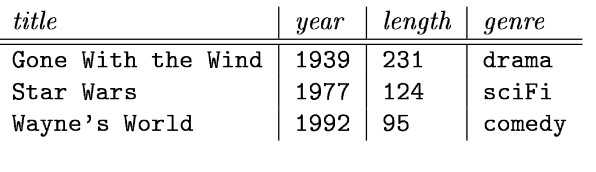
\includegraphics[width=10cm]{reading assignment notes/movie_realtion.jpg}
\item the name of columns are called attributes, in the above relation they are year length and genre
\item a schema is the name of a relation and its set of attributes for the movie relation that is Movies(title,year,length,genre)
\item the attributes of a schema are a set however, the ordering does mater for the purposes of discussion. 
\item a database consists of one or more relations the set of schema for the relations of a database are classed the database schema. 
\item tuples are all the rows of a relation (except for the header which holds attributes) they are normally written as (x,y,z) where x,y,z are the elements of three attributes from the same row
\item the relational model requires that each element of a tuple must be atomic that is of an elementary type (such as int or string) that can not be broken down further into parts so it can not be something like a list
\item each column has a domain ie an atomic type that all elements much adhere to for instance all elements of the movie title column must be strings 
\item sometimes the domain or data type is also included in a schema
\item relations are a set of tuples not a list of tuples so the order does not matter. the same is true for the attributes which can be reordered as we want (however naturally when doing so the order of the columns also change and thus so does the order of all the tuples)
\item a non static relation allows for rows to be added modified or deleted. we can also add or delete attributes but doing so may be expensive or difficult
\item the set of tuples in a relation are called an instance of that relation 
\item typically a database only holds one instance of a relation at a time called the current instance 
\subsection{keys of relations}
\item a fundamental constraint for relational database systems is the key constraint. A set of attributes form a key in a relation if we do not allow two tuples in that relation instance to have the same value in all attributes of the key. 
\item for instance in the movie relation title and year could form a key. that is we don't think two movies should come out the same year with the same name, this however does allow for both multiple movies to come out in one year and for remakes that use the same name 
\item in a schema we indicate the attributes that form a key by underling them for instance in the example above the schema of the movie table would be Movies(\underline{title}, \underline{year}, length,genre)
\item note that the key has to hold for all instances of a relation ie we can not add tuples that violate it. 
\item many real world applications just use artificial keys like movie id. or employee id.
\section{defining a relation schema in SQL}
\item the most common language used to describe and manipulate relational databases is SQL
\item sql has two parts 1. the data definition for declaring database schemes and 2. the data manipulation sub language for queries and modifying a database
\subsection{relations in SQL}
\item sql has three kinds of relations 
\begin{itemize}
    \item stored relations called tables can be changed and viewed
    \item views relations that are not stored but constructed by computation 
    \item temporary tables which are constructed by SQL language processor when a task is preformed and then they are thrown away. 
\end{itemize}
\item the primitive data types of sql
\begin{itemize}
    \item character strings of fixed or varying lengths 
    \item bit strings of fixed or varying length that are similar to character strings but stored as bits
    \item Boolean logical values can take on true false or unknown  
    \item int holding integer values 
    \item floats which hold floating point numbers
    \item DATE and Time objects they are essentially character strings with a restricted form 
\end{itemize}
\item the simplest way to create a table is with the create table key word followed by the name of the relation and coma separated list of attribute names and there types CREATE TABLE movie( title Char(100), year Int);
\item a relation r can be delete by DROP TABLE r
\item alter table allows for an existing relation to be modified ALTER TABLE ADD allows for an attribute to be added. ALTER TABLE DROP allows for an existing attribute to be deleted
\item after declaring an attribute in a schema we can use the DEFAULT command followed by some value to set a default value for that column, which will fill when a row is created with no data in that column. 
\item when adding an attribute you can use the PRIMARY KEY or UNIQUE command to list an attribute as a key. doing so adds the attribute as a key meaning a row can not have all the same values for the keys, and if it is a primary key not tuple can have that value be null
\item pick up at the top of section 2,4 
\section{an algebraic query language}
\item in relational algebra variables are relations constants are finite relations 
\item classes of relational algebra operations 
\begin{itemize}
    \item the set operators union, intersections and differences applies to relations
    \item operations that remove part of a relations. a selection eliminate some rows a projection eliminates some columns. 
    \item operations that combine the tuples of two relations including the Cartesian product and joins
    \item the renaming operation which does not effect the relation its self but changes its schema
\end{itemize}
\subsection{set operations on relations}
\item $R\CUP S$ is the union of the relation R and S is set the set of elements that are present in one of the sets
\item $R\cap S$ is the intersection ie the elements that are in both R and S
\item $R-S$ is the difference of R and S, is the set of elements that are in R but not in S. Note that $R-S\neq S-R$
\item we also put the following two conditions on R and S 
\begin{itemize}
    \item R and S must have Schemas with identical sets of attributes and the type of each attribute must be the same 
    \item the order of attributes in each relation must be the same 
\end{itemize}
\item we can use the rename operator to rename the attributes of a relation allowing for set operations 
\subsection{projection and selection}
\item the projection operator is used to produce from a relation R and new relation that has only some or R's columns 
\item given a relation A with columns $c_1...c_n$ we can write a projection of A with only the first k columns as $\pi_{c_1,...,c_k}(A)$
\item the selection operator applies to a relation R produces a new relation with a subset of R's tuples that satisfy some condition C 
\item this operation is denotes as $\sigma_{c}(R)$
\item  for example if we wanted to select tuples from the relation movie with the attribute length greater than 100 we could write a select as $\sigma_{length>100}(movies)$
\subsection{Cartesian product}
\item the Cartesian product or cross product or just product of two sets R and S written as $R\Times S$ is combination of all pairs of elements in R and S 
\subsection{natural joins}
\item instead of taking a product we most often want to join to tables by only the pairs of tuples that match a condition in some way
\item the natural product written as $S \bowtie R$ of two relations R and S in which we pair only those tuples form R and S that agree in whatever attributes are common to the schemes of R and S
\item let $A_1...A_n$ be all attributes that are in both the schema of R and the schema of S. then a tuple r from R and a tuple S from S are successfully paired if and only if r and s agree on each attribute $A_1...A_n$ if these tuples r,s are successfully paired with a natural join then the result is called a jointed tuple. this joined tuple will agree with tuple r in each attribute of the schema R, as well as each attribute of s in the schema S
\item here is an example of a natural join 
\item 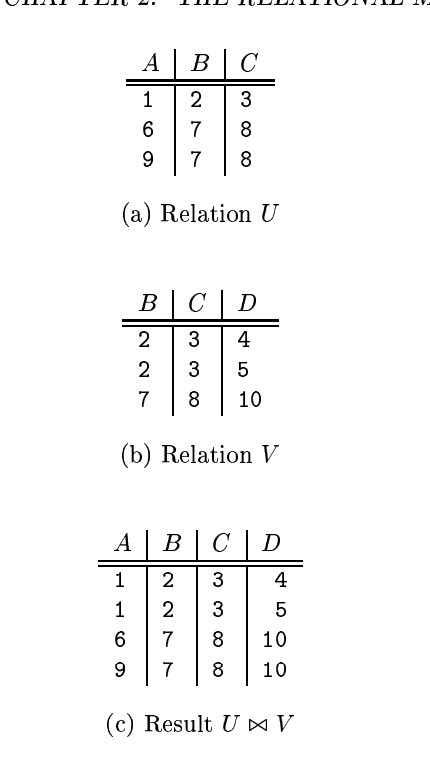
\includegraphics[width=5cm]{reading assignment notes/week 1/database systems the complete book chapter 2/natural_join.jpg}
\subsection{theta joins}
\item the natural join allows us to join two tables on the condition that there attributes agree, we can expand this join to other artistry conditions $\theat$ with the theta join
\item the notation for the theta join on relations R and S based on condition C is $R\bowtie_{C}S$ the result is constructed as follows
\begin{itemize}
    \item take the product of R and s 
    \item select from the product only tuples that satisfy the condition C
\end{itemize}
\item here is an example of a theta join with the condition that the value of attribute A must be less than that of attribute D
\item 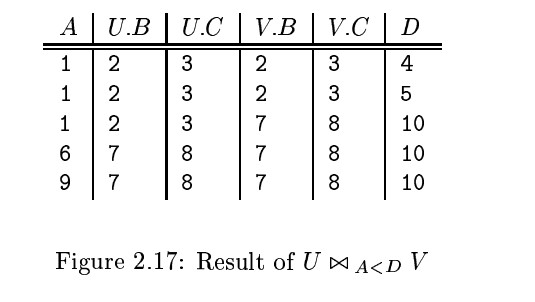
\includegraphics[width=5cm]{reading assignment notes/week 1/database systems the complete book chapter 2/natural_join_2.jpg}

\section{}{combining operations to form queries}
\item we can make more complex commands by chaining together multiple operations 
\subsection{example}
\item suppose we want to know what are the titles and years of movies made by fox that are at least 100 minutes long. 
\item then we select movies with a name long than 100, select movies with studio name= fox compute the intercity of those two selects and take the projection onto attributes title and year
\item 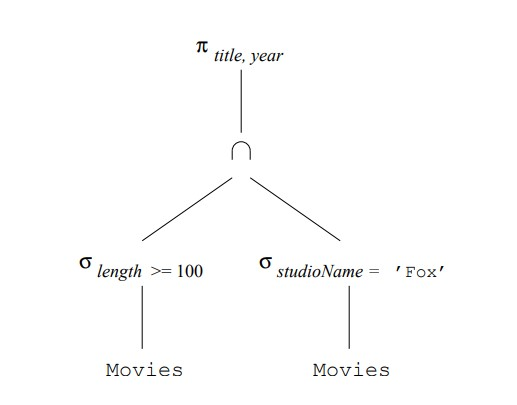
\includegraphics[width=5cm]{reading assignment notes/week 1/database systems the complete book chapter 2/relational_algebra_1.jpg}
witch can aslo be wrirten as \\$\pi_{title,year}(\sigma_{lenght>100}(movies) \cap \sigma_{studioname='fox'}(movies))\\$ or as $\pi_{title,year}(\sigma_{lenght>100}(movies) AND \sigma_{studioname='fox'}(movies))$
\subsection{naming and renaming}
\item to rename a relation R with to S we could do $\rho_{S(A_1...A_N)}(R)$ the relation R now is called S and has attributes $A_1..A_N$ but none of the tuples were changes
\subsection{linear notation for algebraic expressions}
\item note that intersection, natural joins and theta joins can be expressed in terms of the other operations. so the six operations that can not be further reduced as union, difference, selection, projection, product and renaming 
\item instead of writing complex queries as a tree or singular line of algebra we can assign intermediate steps names. 
\item here is an example on the same problem shown above \item 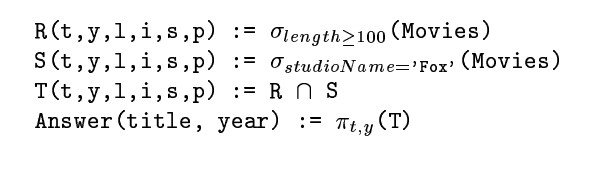
\includegraphics[width=5cm]{reading assignment notes/week 1/database systems the complete book chapter 2/assigment_1.jpg}
\section{constraints on relations}
\item we now turn to the third aspect of a data model the ability to restrict the data that may be stored in a database
\item we are going to express constraints with relational algeba
\section{referential integrity constraints}
\itema common kind of constants referential integrity constraints assert that a value appearing in one context also appear in another related context. 
\item in general if we have any value v as the component in attribute A of some tuple in one relation R then we may except that v will appear Ina  a patricidal compo net say attribute B of some tuple in another relation S this can be expressed as $\pi_{A}(R)\subseteq \pi_{B}(S)$ or equivalently $\pi_{A}(R)-\pi_{B}(S)=\emptyset$
\item this is really just saying that we expect all values in the attribute of A of the relation R to be in the Attribute of B of the relation S, which is equivalent to saying there should be no elements that just appear in the A attribute of R and not in the B attribute of S. 
\subsection{key constants}
\item recall that the key of a relation, is an attribute such that if two tuples have the same value of attributes they must agree on all other attributes 
\item so if there a relation Movie star with key name, then we known as the key is name no tuple can have the same value for name and a different value for any column including address. so we could specifies that name is a key algebraic as $\sigma_{ms1.name=mse2.name and ms1.adress\neq ms2.adress}(MS1\times MS2)=\emptyset$  
\item where MS1 and MS@ are both the movie star set 
\item many other constraints can be constructed from this format. 
\end{itemize}
\end{document}
